\documentclass[12pt,a4paper]{article}

% Essential packages
\usepackage{graphicx}
\usepackage{setspace}
\usepackage[numbers,sort&compress]{natbib}
\usepackage[english]{babel}
\usepackage[utf8]{inputenc}
\usepackage{color}
\usepackage{hyperref}
\usepackage{amsmath,amssymb}
\usepackage{geometry}
\usepackage{longtable}
\usepackage{caption}
\usepackage{tikz}
\usepackage{adjustbox}
\usepackage{listings}
\usepackage{xcolor}
\usepackage{booktabs}
\usepackage{multirow}
\usepackage{float}
\usepackage{subcaption}
\usetikzlibrary{arrows.meta, positioning, shapes.geometric, calc, fit, backgrounds}

% Code listing configuration
\lstset{
    basicstyle=\ttfamily\small,
    breaklines=true,
    frame=single,
    backgroundcolor=\color{gray!10},
    keywordstyle=\color{blue},
    commentstyle=\color{green!50!black},
    stringstyle=\color{red!60!black},
    numbers=left,
    numberstyle=\tiny\color{gray},
    numbersep=5pt,
    showstringspaces=false,
    tabsize=2
}

\lstdefinelanguage{Python}{
    keywords={def, class, return, if, else, elif, for, while, with, as, import, from, async, await, try, except, finally, raise, True, False, None, and, or, not, in, is, lambda, yield},
    keywordstyle=\color{blue}\bfseries,
    ndkeywords={self, cls, BaseModel, Field, Literal, Optional, Union, list, dict, str, int, float, bool},
    ndkeywordstyle=\color{purple},
    sensitive=true,
    comment=[l]{\#},
    morestring=[b]",
    morestring=[b]',
}

% Margin settings
\geometry{
    a4paper,
    left=3cm,
    right=2.5cm,
    top=2.5cm,
    bottom=2.5cm
}

% Hyperref configuration
\hypersetup{
    colorlinks=true,
    linkcolor=blue,
    citecolor=blue,
    urlcolor=blue,
    pdftitle={Materials and Methods - Multi-Agent System for Fact-Checking},
    pdfauthor={Begoña Echavarren Sánchez}
}

% Spacing
\onehalfspacing

\begin{document}

\begin{titlepage}
    \begin{center}
    \vspace*{0.5cm}

    \includegraphics[width=0.6\textwidth]{../../assets/uoc_logo.png}

    \vspace{1.5cm}

    {\Huge \textbf{Materials, Methods and Results}}

    \vspace{2cm}

    {\LARGE \textbf{Multi-Agent System for Automated Fact-Checking of YouTube Videos}}

    \vspace{2.5cm}

    \textbf{\large Begoña Echavarren Sánchez}

    \vspace{0.5cm}

    \textit{Tutor: Josep-Anton Mir Tutusaus}

    \vspace{2cm}

    {\large Master's Degree in Data Science}

    {\large Universitat Oberta de Catalunya}

    \vspace{1cm}

    {\large PEC 3 - Implementation}

    \vspace{0.5cm}

    {\large December 2025}

    \end{center}
\end{titlepage}

\newpage
\pagenumbering{arabic}

\hypersetup{linkcolor=black}
\tableofcontents
\hypersetup{linkcolor=blue}

\newpage

%%%%%%%%%%%%%%%%%%%%%%%%%%%%%%%%%%%%%%%%%%%%%%%%%%%%%%%
% SECTION 1: MATERIALS AND METHODS
%%%%%%%%%%%%%%%%%%%%%%%%%%%%%%%%%%%%%%%%%%%%%%%%%%%%%%%
\section{Materials and Methods}

This section presents the comprehensive technical implementation of Factible, a multi-agent system for automated fact-checking of YouTube videos. The system implements an end-to-end pipeline that processes video content through five specialized components, leveraging large language models (LLMs) for reasoning tasks while employing classical algorithms for deterministic operations. The implementation follows design-science principles \citep{hevner2004design, oates2006researching}, emphasizing the creation of artifacts that extend human capabilities through systematic evaluation and iterative refinement.

%-------------------------------------------------------
\subsection{System Architecture Overview}
%-------------------------------------------------------

\subsubsection{High-Level Architecture}

Factible implements an end-to-end automated fact-checking pipeline for YouTube videos using a multi-agent architecture. Recent research on LLM agents demonstrates that multi-agent collaboration can enhance factuality and reasoning by allowing specialized agents to converse and coordinate on tasks \citep{wu2023autogen}. FactAgent further shows that decomposing fact-checking into dedicated agents for input ingestion, query generation, evidence retrieval, and verdict prediction yields higher accuracy and transparency \citep{zhang2025factagent}. The Factible architecture follows this line of work by processing video content through five specialized, modular components that operate sequentially with four levels of internal parallelization.

The system processes a YouTube video URL through the following stages:

\begin{enumerate}
    \item \textbf{Transcriptor}: Extracts video transcript via YouTube Transcript API, preserving timestamped segments for claim localization, with automatic fallback to proxy service when rate-limited.

    \item \textbf{Claim Extractor} (LLM Agent): Employs thesis-first reasoning to infer the video's central argument, extracts factual and verifiable claims with importance scoring, and performs post-processing through fuzzy matching to locate claims in transcript positions.

    \item \textbf{Query Generator} (LLM Agent): Generates diverse search queries across four types (direct, alternative, source-seeking, and contextual), assigns priority scores based on evidence likelihood, and filters by priority threshold and budget constraints.

    \item \textbf{Online Search}: Executes a multi-step pipeline including Google Search via Serper API, website reliability assessment using Media Bias/Fact Check (MBFC) data combined with heuristics \citep{mbfc2024methodology}, content fetching via Selenium WebDriver, and LLM-based evidence extraction with stance classification.

    \item \textbf{Output Generator} (LLM Agent): Builds evidence bundles grouped by stance, generates verdicts with confidence levels, calculates algorithmic evidence quality scores, and maps claims to video timestamps for user interface navigation.
\end{enumerate}

Figure \ref{fig:pipeline-architecture} illustrates the complete pipeline architecture with data flow and parallelization points.

\begin{figure}[H]
\centering
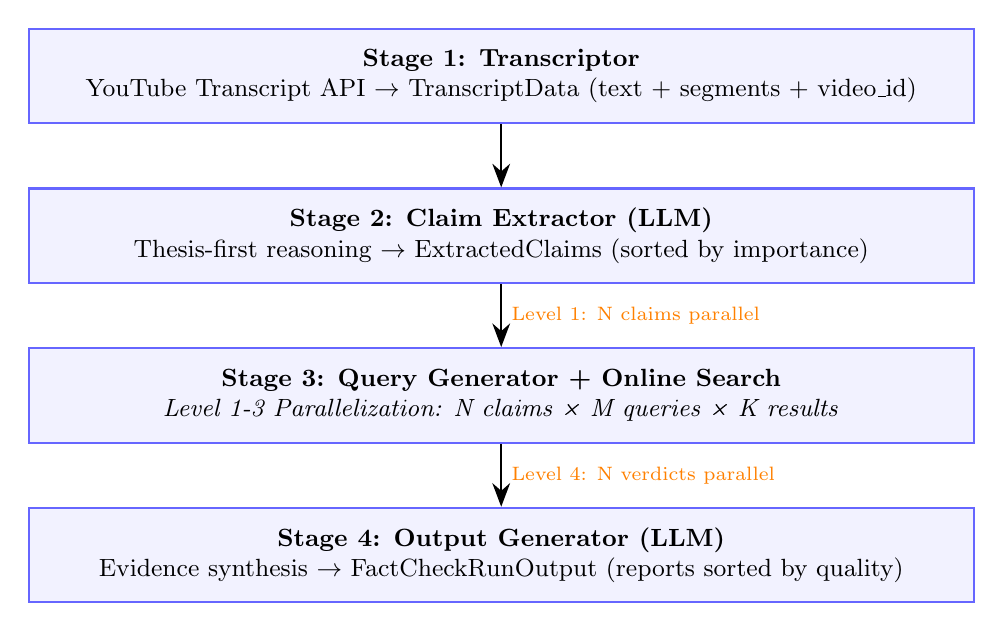
\begin{tikzpicture}[
    node distance=0.8cm,
    box/.style={rectangle, draw=blue!60, fill=blue!5, thick, minimum width=12cm, minimum height=1.2cm, align=center, font=\small},
    arrow/.style={-{Stealth[length=3mm]}, thick},
    parallel/.style={draw=orange!70, dashed, thick}
]

% Stage 1
\node[box] (s1) {
    \textbf{Stage 1: Transcriptor}\\
    YouTube Transcript API $\rightarrow$ TranscriptData (text + segments + video\_id)
};

% Stage 2
\node[box, below=of s1] (s2) {
    \textbf{Stage 2: Claim Extractor (LLM)}\\
    Thesis-first reasoning $\rightarrow$ ExtractedClaims (sorted by importance)
};

% Stage 3
\node[box, below=of s2] (s3) {
    \textbf{Stage 3: Query Generator + Online Search}\\
    \textit{Level 1-3 Parallelization: N claims × M queries × K results}
};

% Stage 4
\node[box, below=of s3] (s4) {
    \textbf{Stage 4: Output Generator (LLM)}\\
    Evidence synthesis $\rightarrow$ FactCheckRunOutput (reports sorted by quality)
};

% Arrows
\draw[arrow] (s1) -- (s2);
\draw[arrow] (s2) -- node[right, font=\scriptsize, orange] {Level 1: N claims parallel} (s3);
\draw[arrow] (s3) -- node[right, font=\scriptsize, orange] {Level 4: N verdicts parallel} (s4);

\end{tikzpicture}
\caption{High-level pipeline architecture showing the four main stages and parallelization levels.}
\label{fig:pipeline-architecture}
\end{figure}

\subsubsection{Design Principles}

The system adheres to several key design principles derived from software engineering best practices and GenAI application development, aligned with the design-science paradigm in information systems research \citep{hevner2004design}:

\begin{enumerate}
    \item \textbf{Modularity}: Each component is isolated with well-defined inputs and outputs using Pydantic schemas, enabling independent optimization, testing, and replacement.

    \item \textbf{Structured Outputs}: All LLM interactions use Pydantic AI with typed output schemas, ensuring type safety, automatic validation, and consistent data structures across the pipeline.

    \item \textbf{Transparency}: The full evidence chain is preserved and exposed to users---sources, reliability ratings, stances, and reasoning are all traceable from final verdict back to original source.

    \item \textbf{Progressive Enhancement}: The pipeline operates with graceful degradation (e.g., fallback to snippet if scraping fails, fallback to proxy if rate-limited) rather than failing entirely.

    \item \textbf{Cost-Conscious Design}: Configurable limits (\texttt{max\_claims}, \texttt{max\_queries}, \texttt{max\_results}) prevent runaway API costs during development and production.

    \item \textbf{Reproducibility}: Deterministic LLM outputs (\texttt{temperature=0.0}), structured YAML configurations, and comprehensive experiment tracking enable reproducible research.

    \item \textbf{Separation of Concerns}: Classical algorithms handle tasks like reliability scoring, deduplication, and quality calculation, reserving LLM calls for tasks requiring reasoning and language understanding.
\end{enumerate}

\subsubsection{Component Isolation Pattern}

Each component follows a consistent directory structure that enables independent testing, model swapping, metrics collection, and clear interface contracts:

\begin{lstlisting}[language=bash, caption={Component directory structure}]
component/
    __init__.py          # Public exports
    component_name.py    # Main logic with @track_pydantic decorator
    schemas.py           # Pydantic models for input/output
\end{lstlisting}

%-------------------------------------------------------
\subsection{Technology Stack}
%-------------------------------------------------------

\subsubsection{Core Technologies}

Table \ref{tab:tech-stack} presents the core technologies employed in the implementation.

\begin{table}[H]
\centering
\caption{Core technology stack}
\label{tab:tech-stack}
\begin{tabular}{llll}
\toprule
\textbf{Category} & \textbf{Technology} & \textbf{Version} & \textbf{Purpose} \\
\midrule
Language & Python & 3.12 & Core implementation with type hints \\
LLM Framework & Pydantic AI & $\geq$1.0.0 & Agent orchestration, structured outputs \\
Data Validation & Pydantic & $\geq$2.0.0 & Schema definitions, runtime validation \\
Web Framework & FastAPI & $\geq$0.115.0 & REST API with SSE streaming \\
HTTP Server & Uvicorn & $\geq$0.32.0 & High-performance ASGI server \\
Async HTTP & httpx & $\geq$0.28.1 & Async HTTP client \\
Web Scraping & Selenium & $\geq$4.15.2 & JavaScript-rendered content extraction \\
YouTube & youtube-transcript-api & $\geq$1.2.2 & Transcript extraction \\
Domain Info & python-whois & $\geq$0.8.0 & Domain age lookup \\
CLI & Typer & $\geq$0.15.0 & Experiment runner CLI \\
Analysis & pandas, matplotlib & - & Data analysis and visualization \\
\bottomrule
\end{tabular}
\end{table}

\subsubsection{Large Language Models}

The system supports multiple LLM providers to enable comparison of cost-quality trade-offs. Table \ref{tab:llm-models} shows the available models and their configurations.

\begin{table}[H]
\centering
\caption{LLM providers and pricing}
\label{tab:llm-models}
\begin{tabular}{lllll}
\toprule
\textbf{Provider} & \textbf{Model} & \textbf{Context} & \textbf{Pricing (per 1M tokens)} & \textbf{Use Case} \\
\midrule
OpenAI & gpt-4o-mini & 128K & \$0.15 / \$0.60 & Default \\
OpenAI & gpt-4o & 128K & \$5.00 / \$15.00 & High-quality \\
OpenAI & gpt-4-turbo & 128K & \$10.00 / \$30.00 & Premium \\
Ollama & qwen3:8b & 40K & Free (local) & Budget/offline \\
Ollama & qwen3:4b & 256K & Free (local) & Small footprint \\
\bottomrule
\end{tabular}
\end{table}

Large language models such as GPT-4 offer multimodal capabilities and demonstrate human-level performance across diverse benchmarks \citep{openai2024gpt4}. Despite these advances, models still suffer from hallucinations and are constrained by limited context windows, underscoring the need for careful configuration and reliability safeguards \citep{openai2024gpt4}. Our model management layer therefore emphasizes deterministic outputs, context-aware trimming, and tool-assisted generation.

\subsubsection{External Services}

The system integrates with external services for search and transcript extraction:

\begin{itemize}
    \item \textbf{Serper API}: Google Search wrapper providing organic search results with approximately 2,500 queries per month on the free tier.
    \item \textbf{YouTube oEmbed API}: Video metadata retrieval without authentication.
    \item \textbf{Webshare Proxy}: Rate limit bypass for transcript extraction with configurable proxy locations.
\end{itemize}

%-------------------------------------------------------
\subsection{Pipeline Components}
%-------------------------------------------------------

\subsubsection{Transcriptor}

The Transcriptor component extracts YouTube video transcripts with precise timestamp information for later claim-to-video mapping.

\paragraph{Implementation Details}

The transcriptor uses the \texttt{youtube-transcript-api} library to fetch available transcripts, with preference for English (\texttt{["en", "en-US"]}). When rate-limited by YouTube, it automatically falls back to a proxy service (Webshare). Key features include:

\begin{itemize}
    \item \textbf{Timestamped Segments}: Each segment preserves \texttt{start} time and \texttt{duration} in seconds.
    \item \textbf{Character Position Mapping}: Enables mapping claim text positions back to video timestamps.
    \item \textbf{Title Fetching}: Uses YouTube oEmbed API to retrieve video title for context.
    \item \textbf{Proxy Fallback}: Automatic retry through Webshare proxy when rate-limited.
\end{itemize}

\paragraph{Output Schema}

\begin{lstlisting}[language=Python, caption={Transcriptor output schemas}]
class TranscriptSegment(BaseModel):
    """A single timestamped segment from a YouTube transcript."""
    text: str = Field(description="The text content of this segment")
    start: float = Field(ge=0.0, description="Start time in seconds")
    duration: float = Field(ge=0.0, description="Duration in seconds")

class TranscriptData(BaseModel):
    """Complete transcript data with timestamped segments."""
    text: str = Field(description="Full transcript as plain text")
    segments: list[TranscriptSegment]
    video_id: str = Field(description="YouTube video ID")
\end{lstlisting}

\paragraph{Timestamp Mapping Algorithm}

The \texttt{map\_char\_position\_to\_timestamp()} function enables the system to locate where in the video each claim originates by iterating through segments and tracking character positions:

\begin{lstlisting}[language=Python, caption={Timestamp mapping algorithm}]
def map_char_position_to_timestamp(
    char_position: int, transcript_data: TranscriptData
) -> dict | None:
    """Map character position in transcript to video timestamp."""
    current_char = 0
    for idx, segment in enumerate(transcript_data.segments):
        segment_text = segment.text + " "
        segment_length = len(segment_text)
        if current_char <= char_position < current_char + segment_length:
            return {
                "segment_index": idx,
                "start": segment.start,
                "duration": segment.duration,
            }
        current_char += segment_length
    return {"start": transcript_data.segments[-1].start, ...}
\end{lstlisting}

%---

\subsubsection{Claim Extractor}

The Claim Extractor identifies factual, verifiable claims from video transcripts using LLM-based extraction with thesis-relative importance ranking. Our approach builds on prior work in automated claim detection: supervised models trained on annotated political debates have been used to detect check-worthy claims \citep{hassan2015claimbuster}, and end-to-end systems like ClaimBuster monitor public discourse and prioritize factual statements for manual fact-checking \citep{li2017claimbuster}. These systems show that focusing on salient, verifiable claims improves the efficiency of fact-checking pipelines.

\paragraph{LLM Configuration}

The claim extractor uses deterministic settings for reproducibility:

\begin{lstlisting}[language=Python, caption={Claim extractor model settings}]
CLAIM_EXTRACTOR_MODEL_SETTINGS: ModelSettings = {
    "temperature": 0.0,    # Deterministic outputs for reproducibility
    "max_tokens": 1200,    # Limit response length to control latency
}
retries = 3  # Automatic retries on LLM failures
\end{lstlisting}

\paragraph{Prompt Engineering Strategy: Thesis-First Approach}

The claim extractor employs a novel \textit{thesis-first approach} with multi-step reasoning designed to prioritize claims most critical to the video's central argument:

\textbf{Step 1: Thesis Inference} --- Before listing claims, the LLM infers the video's central thesis in no more than 25 words (e.g., ``Climate change alarmism is driven more by politics and media than by settled science'').

\textbf{Step 2: Importance Ranking with Thesis Impact Test} --- Claims are scored based on their impact on the video's thesis using the question: ``If this claim were proven false, would the thesis collapse or materially weaken?'' Table \ref{tab:importance-scoring} presents the scoring guidelines.

\begin{table}[H]
\centering
\caption{Claim importance scoring guidelines}
\label{tab:importance-scoring}
\begin{tabular}{lll}
\toprule
\textbf{Score Range} & \textbf{Description} & \textbf{Examples} \\
\midrule
0.85--1.0 & Prescriptive/causal claims undermining thesis & Policy proposals, causal mechanisms \\
0.60--0.80 & Quantitative/historical evidence tied to thesis & Statistics, dates, expert citations \\
0.30--0.55 & Context/supporting background & Definitions, general facts \\
0.0--0.25 & Peripheral/anecdotal details & Personal stories, credentials \\
\bottomrule
\end{tabular}
\end{table}

\textbf{Step 3: Relevance Guardrails} --- Pure credential facts are capped at 0.30 unless the thesis questions expertise; statements not affecting the thesis are capped at 0.25; pure opinions are excluded; and paraphrases and duplicate numbers are removed.

\paragraph{Dynamic Instructions via Pydantic AI Dependencies}

The agent uses Pydantic AI's dependency injection and \texttt{@agent.instructions} decorator to inject runtime constraints:

\begin{lstlisting}[language=Python, caption={Dynamic instruction injection}]
class ClaimExtractorDeps(BaseModel):
    max_claims: int | None = None

@agent.instructions
def _limit_instruction(ctx: RunContext[ClaimExtractorDeps]) -> str:
    """Dynamically inject max_claims constraint into system prompt."""
    max_claims = ctx.deps.max_claims
    if max_claims is not None and max_claims >= 0:
        return f"Never output more than {max_claims} claims."
    return "Output only the highest-impact claims."
\end{lstlisting}

\paragraph{Post-Processing: Fuzzy Claim Localization}

After LLM extraction, each claim is located in the original transcript using fuzzy string matching. The algorithm normalizes text, applies a sliding window with $\pm 2$ words around the claim length, computes similarity using \texttt{difflib.SequenceMatcher}, and requires a minimum score of 0.5 for a match. This produces \texttt{transcript\_char\_start}, \texttt{transcript\_char\_end}, and \texttt{transcript\_match\_score} fields for timestamp mapping.

\paragraph{Output Schema}

\begin{lstlisting}[language=Python, caption={Claim extractor output schemas}]
class Claim(BaseModel):
    """A single claim or fact extracted from text."""
    text: str  # Claim text (<=40 words recommended)
    confidence: float = Field(ge=0.0, le=1.0)
    category: str  # historical, scientific, statistical, etc.
    importance: float = Field(default=0.5, ge=0.0, le=1.0)
    context: str | None = Field(default=None)
    # Post-processing fields
    transcript_char_start: int | None = None
    transcript_char_end: int | None = None
    transcript_match_score: float | None = None

class ExtractedClaims(BaseModel):
    """Collection of claims extracted from a transcript."""
    claims: list[Claim]  # Sorted by importance (descending)
    total_count: int
\end{lstlisting}

Standard fact-checking datasets such as FEVER \citep{thorne2018fever} and FEVEROUS \citep{aly2021feverous} are used as external references to evaluate claim extraction performance. FEVER contains 185,445 claims derived from Wikipedia sentences labeled as Supported, Refuted, or NotEnoughInfo, while FEVEROUS extends this to 87,026 claims with both unstructured text and structured table evidence.

%---

\subsubsection{Query Generator}

The Query Generator produces diverse, prioritized search queries optimized for evidence retrieval. Research on LLMs shows that interleaving reasoning and acting enables models to plan and perform external searches more effectively; the ReAct prompting technique encourages models to produce intermediate reasoning steps and task-specific actions, leading to improved factuality and reduced hallucination \citep{yao2023react}. Retrieval-augmented generation methods combine parametric language models with non-parametric memory to retrieve relevant documents \citep{lewis2020retrieval}, while frameworks like RARR perform post-generation research and revision to align outputs with supporting evidence \citep{gao2022rarr}.

\paragraph{Query Type Taxonomy}

The system generates four types of queries with different search strategies, as shown in Table \ref{tab:query-types}.

\begin{table}[H]
\centering
\caption{Query type taxonomy}
\label{tab:query-types}
\begin{tabular}{llll}
\toprule
\textbf{Type} & \textbf{Description} & \textbf{Strategy} & \textbf{Example} \\
\midrule
DIRECT & Exact claim phrasing & Verbatim search & ``unemployment rose 15\% Q3 2024'' \\
ALTERNATIVE & Rephrased with synonyms & Semantic variation & ``jobless rate increase third quarter'' \\
SOURCE & Target authoritative sources & Source-seeking & ``BLS unemployment statistics Q3'' \\
CONTEXT & Broader context & Background search & ``economic indicators fall 2024'' \\
\bottomrule
\end{tabular}
\end{table}

\paragraph{Priority System}

Queries are prioritized 1--5 based on likelihood of finding reliable, definitive information: priority 1 queries are always included, priority 2 by default, priority 3 if budget allows, and priorities 4--5 rarely or only for completeness.

\paragraph{Output Schema}

\begin{lstlisting}[language=Python, caption={Query generator output schemas}]
class SearchQuery(BaseModel):
    query: str           # Search query text
    query_type: str      # "direct", "alternative", "source", "context"
    priority: int        # 1-5 (1 = highest priority)

class GeneratedQueries(BaseModel):
    original_claim: str           # Reference to source claim
    queries: list[SearchQuery]    # Filtered and sorted queries
    total_count: int              # Original count before filtering
\end{lstlisting}

%---

\subsubsection{Online Search}

The Online Search component implements a multi-step pipeline to retrieve, assess, and extract evidence from web sources with adaptive quality filtering. The reliability assessment combines domain-level heuristics with the Media Bias/Fact Check (MBFC) methodology, which employs a comprehensive weighted scoring system to evaluate media outlets' ideological bias and factual reliability \citep{mbfc2024methodology}. To mitigate hallucinations and ensure evidence quality, we draw on research like SelfCheckGPT, which detects hallucinations by comparing multiple sampled responses and ranks passages by factuality \citep{manakul2023selfcheckgpt}. Our multi-agent retrieval strategy is further informed by systems such as FactAgent \citep{zhang2025factagent} and LoCal \citep{chen2024local}, where decomposing, reasoning, and evaluating agents iteratively refine answers and outperform baselines.

\paragraph{Step 1: Google Search (Serper API)}

The Google search client wraps the Serper API for asynchronous search execution:

\begin{lstlisting}[language=Python, caption={Google search client implementation}]
class GoogleSearchClient:
    """Wrapper around the Google Serper search API."""

    async def search(self, query: str, limit: int = 5) -> list[GoogleSearchHit]:
        """Execute async search with connection reuse."""
        client = await self._get_client()
        response = await client.post(
            "https://google.serper.dev/search",
            headers={"X-API-KEY": self.api_key},
            json={"q": query, "num": min(limit, 10)},
        )
        raw_results = response.json().get("organic", [])
        return [GoogleSearchHit(title=r["title"], url=r["link"],
                                snippet=r["snippet"])
                for r in raw_results[:limit]]
\end{lstlisting}

\paragraph{Step 2: Website Reliability Assessment}

The reliability checker uses a multi-factor scoring system with first-match priority:

\textbf{Factor 1: Media Bias/Fact Check (MBFC) Dataset} --- The system loads timestamped JSON snapshots containing over 10,000 news sources with credibility ratings. Credibility mappings are: high $\rightarrow$ 0.85, medium $\rightarrow$ 0.60, low $\rightarrow$ 0.30, very low $\rightarrow$ 0.15.

\textbf{Factor 2: TLD Reputation} --- High-trust top-level domains (\texttt{.gov}, \texttt{.edu}, \texttt{.int}) receive a 0.90 score.

\textbf{Factor 3: Domain Age via WHOIS} --- Domains $\geq$10 years old receive a +0.10 bonus, while domains $<$1 year old receive a --0.15 penalty.

\begin{lstlisting}[language=Python, caption={Reliability assessment output schema}]
class SiteReliability(BaseModel):
    """Assessment of a website's reliability."""
    rating: Literal["high", "medium", "low", "unknown"]
    score: float = Field(ge=0.0, le=1.0)
    reasons: list[str] = Field(default_factory=list)
    bias: str | None = None  # Political bias if available
\end{lstlisting}

\paragraph{Step 3: Content Fetching (Selenium)}

Content fetching uses Selenium WebDriver in headless Chrome mode with smart wait strategies to handle JavaScript-heavy sites:

\begin{lstlisting}[language=Python, caption={Selenium content fetcher configuration}]
class SeleniumContentFetcher:
    def __init__(self, headless: bool = True, wait_timeout: int = 12,
                 page_load_timeout: int = 20, max_characters: int = 8000):
        chrome_options = Options()
        if headless:
            chrome_options.add_argument("--headless=new")
        chrome_options.add_argument("--disable-gpu")
        chrome_options.add_argument("--no-sandbox")
        chrome_options.add_argument("--blink-settings=imagesEnabled=false")
\end{lstlisting}

The fetcher first attempts a quick extraction of paragraph elements; if content is insufficient ($<$100 characters), it waits for JavaScript rendering before retrying. Content is trimmed to a maximum of 8,000 characters. Async integration wraps blocking Selenium calls in \texttt{asyncio.to\_thread()} for non-blocking operation.

\paragraph{Step 4: Evidence Extraction (LLM)}

The evidence extractor analyzes retrieved content against claims using structured stance definitions:

\begin{itemize}
    \item \textbf{SUPPORTS}: Evidence confirms or validates the claim through direct statements, semantic equivalents, or mechanism descriptions.
    \item \textbf{REFUTES}: Evidence contradicts or disproves the claim through counter-evidence or statements that evidence is unproven/disproven.
    \item \textbf{MIXED}: Both supporting and refuting elements present.
    \item \textbf{UNCLEAR}: Genuinely ambiguous content that discusses related topics without addressing the specific claim.
\end{itemize}

Critical prompt instructions ensure that mere discussion equals UNCLEAR, that mechanisms are recognized even without exact terminology, and that both Google snippets and page content are considered with better evidence prioritized.

\paragraph{Adaptive Credibility Filtering}

The search orchestrator implements adaptive credibility filtering as a key innovation for ensuring evidence quality:

\begin{lstlisting}[language=Python, caption={Adaptive credibility filtering algorithm}]
async def search_online_async(claim: str, query: str, limit: int = 5,
                              min_credibility: str = "medium") -> SearchResults:
    # Step 1: Fetch initial batch (2x limit for filtering headroom)
    batch_1 = await search_client.search(query, limit=limit * 2)

    # Step 2: Quality check - if >50% unreliable, fetch more
    reliable_count = sum(1 for _, score, _ in all_assessed if score >= min_score)
    if reliable_count < len(all_assessed) / 2:
        batch_2 = await search_client.search(query, limit=limit * 2)

    # Step 3: Intelligent filtering with minimum guarantee
    all_assessed.sort(key=lambda x: x[1], reverse=True)
    if len(reliable) >= min_guaranteed_sources:
        filtered_results = reliable[:limit * 2]
    else:
        needed = min_guaranteed_sources - len(reliable)
        filtered_results = reliable + unreliable[:needed]
\end{lstlisting}

Additional filtering includes stance filtering (removing unclear results if $>$50\% have definitive stances) and URL deduplication using hash sets.

%---

\subsubsection{Output Generator}

The Output Generator synthesizes evidence into coherent verdicts with confidence levels, quality scoring, and timestamp mapping.

\paragraph{Two-Step Process}

\textbf{Step 1: Build Evidence Bundle (Algorithmic)} --- The system groups, deduplicates, and sorts evidence by stance. Within each stance group, sources are sorted by reliability (high first), then by score, with alphabetic tie-breaking.

\textbf{Step 2: Generate Verdict (LLM)} --- Evidence is formatted for the LLM prompt with stance, source count, reliability, and summaries. The system prompt instructs concise synthesis, naming sources only when clarifying contrasting perspectives, and explicitly naming supporting and refuting sources when evidence conflicts.

\paragraph{Evidence Quality Score (Algorithmic)}

The quality score is calculated algorithmically without LLM involvement for consistency and speed:

\begin{lstlisting}[language=Python, caption={Evidence quality score calculation}]
def _calculate_evidence_quality_score(bundle: ClaimEvidenceBundle) -> float:
    """Quality score from 0.0 (no evidence) to 1.0 (high-quality evidence)."""
    if bundle.total_sources == 0:
        return 0.0

    score = 0.3  # Base score for having any evidence

    # Bonus for actionable stances (supports/refutes/mixed)
    actionable_count = sum(len(sources) for stance, sources
                          in bundle.stance_groups.items()
                          if stance in ("supports", "refutes", "mixed"))
    score += 0.3 * min(1.0, actionable_count / 3.0)

    # Bonus for high/medium reliability sources
    high_reliability_count = sum(1 for sources in bundle.stance_groups.values()
                                 for source in sources
                                 if source.reliability.rating in ("high", "medium"))
    score += 0.4 * min(1.0, high_reliability_count / 3.0)

    return min(1.0, score)
\end{lstlisting}

Table \ref{tab:quality-score} summarizes the quality score components.

\begin{table}[H]
\centering
\caption{Evidence quality score breakdown}
\label{tab:quality-score}
\begin{tabular}{lll}
\toprule
\textbf{Component} & \textbf{Weight} & \textbf{Criteria} \\
\midrule
Base & 0.3 & Having any evidence \\
Actionable & 0.3 & Up to 3 supports/refutes/mixed sources \\
Reliability & 0.4 & Up to 3 high/medium reliability sources \\
\textbf{Maximum} & \textbf{1.0} & \\
\bottomrule
\end{tabular}
\end{table}

\paragraph{Parallel Verdict Generation (Level 4)}

All verdicts are generated concurrently using \texttt{asyncio.gather()}:

\begin{lstlisting}[language=Python, caption={Parallel verdict generation}]
async def generate_run_output(...) -> FactCheckRunOutput:
    """Generate all verdict reports in parallel."""
    report_tasks = [
        _generate_report_with_context(idx, claim, results)
        for idx, (claim, results) in enumerate(claim_results, 1)
    ]
    reports = await asyncio.gather(*report_tasks)
    sorted_reports = sorted(reports,
                           key=lambda r: r.evidence_quality_score,
                           reverse=True)
    return FactCheckRunOutput(claim_reports=sorted_reports, ...)
\end{lstlisting}

\paragraph{Output Schema}

\begin{lstlisting}[language=Python, caption={Output generator schemas}]
VerdictConfidence = Literal["low", "medium", "high"]

class ClaimFactCheckReport(BaseModel):
    """Structured report ready to present to end users."""
    claim_text: str
    claim_confidence: float
    claim_category: str
    overall_stance: EvidenceStance
    verdict_confidence: VerdictConfidence
    verdict_summary: str
    evidence_by_stance: dict[EvidenceStance, list[EvidenceSourceSummary]]
    total_sources: int = Field(ge=0)
    evidence_quality_score: float = Field(ge=0.0, le=1.0)
    timestamp_hint: float | None = None
    timestamp_confidence: float | None = None
\end{lstlisting}

%-------------------------------------------------------
\subsection{LLM Configuration and Model Management}
%-------------------------------------------------------

\subsubsection{Model Abstraction Layer}

The system uses an enum-based model configuration with Pydantic validation for type-safe model management:

\begin{lstlisting}[language=Python, caption={Model configuration abstraction}]
class ModelConfig(BaseModel):
    """Configuration for a language model including provider and pricing."""
    provider: str  # "openai" or "ollama"
    model_name: str
    price_input_per_million: float
    price_output_per_million: float
    context_window: int

class ModelChoice(Enum):
    """Available language models with their configurations."""
    OPENAI_GPT4O_MINI = ModelConfig(
        provider="openai", model_name="gpt-4o-mini",
        price_input_per_million=0.150,
        price_output_per_million=0.600, context_window=128_000)
    # ... additional models
\end{lstlisting}

\subsubsection{Model Instantiation with Caching}

Ollama model instances are cached using \texttt{@lru\_cache} for connection reuse:

\begin{lstlisting}[language=Python, caption={Model instantiation with caching}]
@lru_cache(maxsize=None)
def _get_ollama_model(model_name: str) -> OpenAIChatModel:
    """Get cached Ollama model instance for connection reuse."""
    provider = OllamaProvider(base_url="http://127.0.0.1:11434/v1")
    return OpenAIChatModel(model_name=model_name, provider=provider)
\end{lstlisting}

\subsubsection{Per-Component Model Configuration}

A centralized configuration enables easy model swapping, per-component optimization, experiment flexibility, and cost tracking:

\begin{lstlisting}[language=Python, caption={Per-component model configuration}]
CLAIM_EXTRACTOR_MODEL = ModelChoice.OPENAI_GPT4O_MINI
QUERY_GENERATOR_MODEL = ModelChoice.OPENAI_GPT4O_MINI
EVIDENCE_EXTRACTOR_MODEL = ModelChoice.OPENAI_GPT4O_MINI
OUTPUT_GENERATOR_MODEL = ModelChoice.OPENAI_GPT4O_MINI
\end{lstlisting}

\subsubsection{Common Model Settings}

All components use \texttt{temperature=0.0} for deterministic outputs, enabling reproducibility, consistency in structured outputs, and meaningful A/B comparisons. Table \ref{tab:model-settings} shows the token limits per component.

\begin{table}[H]
\centering
\caption{Component model settings}
\label{tab:model-settings}
\begin{tabular}{llll}
\toprule
\textbf{Component} & \textbf{Temperature} & \textbf{Max Tokens} & \textbf{Rationale} \\
\midrule
Claim Extractor & 0.0 & 1,200 & Deterministic, structured claims \\
Query Generator & 0.0 & 600 & Concise queries, no explanations \\
Evidence Extractor & 0.0 & 1,100 & Summary + key quote \\
Output Generator & 0.0 & 900 & Concise verdict synthesis \\
\bottomrule
\end{tabular}
\end{table}

%-------------------------------------------------------
\subsection{Latency Optimization Strategies}
%-------------------------------------------------------

The system implements multiple latency optimization strategies. Research into LLM latency shows that prompt size, completion length, and model size are the dominant factors in inference time; reducing input and output token counts directly lowers compute and memory overhead \citep{graphsignal2024latency}. Additional techniques such as defining clear output boundaries, setting token limits, and adjusting sampling temperature can reduce generated tokens \citep{graphsignal2024latency}, and caching prompts allows reuse of computations for identical prefixes. Choosing smaller model weights yields faster inference speeds.

\subsubsection{Process Tokens Faster: Model Selection}

The default model (gpt-4o-mini) balances speed, cost-effectiveness, and 128K context. Local Ollama models provide budget and offline options.

\subsubsection{Generate Fewer Tokens: Output Constraints}

Each component has carefully tuned \texttt{max\_tokens} limits: claims limited to 40 words, context to 20 words, evidence summaries to 1--2 sentences.

\subsubsection{Use Fewer Input Tokens: Content Trimming}

Web content is trimmed to 6,000--8,000 characters; evidence prompts include only snippets and page content (not raw HTML).

\subsubsection{Make Fewer Requests: Combined Operations}

Single LLM calls per component with no multi-turn conversations; batch generation produces all queries in one call; single synthesis calls with all evidence per claim.

\subsubsection{Parallelize: 4-Level Async Architecture}

The system implements four levels of parallelization:

\begin{itemize}
    \item \textbf{Level 1}: Process N claims in parallel using \texttt{asyncio.gather}
    \item \textbf{Level 2}: For each claim, process M queries in parallel
    \item \textbf{Level 3}: For each query, process K results in parallel (reliability assessment, content fetching, and evidence extraction)
    \item \textbf{Level 4}: Generate all N verdicts in parallel
\end{itemize}

Blocking I/O operations (Selenium, WHOIS) are wrapped in \texttt{asyncio.to\_thread()} to avoid blocking the event loop.

\subsubsection{Real-Time Streaming}

Server-Sent Events (SSE) provide progressive updates as the pipeline executes, with progress stages from 5\% (transcript extraction) through 100\% (complete). Claims are shown immediately after extraction, before search completes.

\subsubsection{Classical Methods for Non-Reasoning Tasks}

Table \ref{tab:classical-methods} shows operations handled by classical algorithms rather than LLMs.

\begin{table}[H]
\centering
\caption{Operations using classical methods}
\label{tab:classical-methods}
\begin{tabular}{lll}
\toprule
\textbf{Operation} & \textbf{Method} & \textbf{Rationale} \\
\midrule
Reliability scoring & Rule-based + MBFC lookup & Faster, deterministic, no API cost \\
Claim localization & Fuzzy string matching & No LLM needed for text search \\
Evidence quality score & Algorithmic calculation & Consistent, fast, reproducible \\
URL deduplication & Hash set & O(1) lookup \\
Stance filtering & Threshold-based & Simple percentage check \\
\bottomrule
\end{tabular}
\end{table}

%-------------------------------------------------------
\subsection{Data Schemas and Structured Outputs}
%-------------------------------------------------------

\subsubsection{Pydantic AI Integration}

All LLM agents use Pydantic models as \texttt{output\_type}, ensuring type safety, automatic parsing, error handling with automatic retries, IDE support with full autocomplete, and serialization via \texttt{model\_dump()}.

\begin{lstlisting}[language=Python, caption={Pydantic AI agent pattern}]
agent = Agent(
    model=get_model(MODEL_CHOICE),
    output_type=ExtractedClaims,  # Pydantic model
    deps_type=ClaimExtractorDeps,  # Runtime dependencies
    model_settings={"temperature": 0.0, "max_tokens": 1200},
    system_prompt="...",
    retries=3,
)
\end{lstlisting}

\subsubsection{Schema Design Principles}

The schema design follows five principles: flat structures to avoid deep nesting; optional fields using \texttt{str | None}; \texttt{Literal} types for constraints; descriptive field names with \texttt{Field} descriptions; and validation constraints such as \texttt{Field(ge=0.0, le=1.0)}.

%-------------------------------------------------------
\subsection{Evaluation Framework}
%-------------------------------------------------------

Evaluating fact-checking systems remains an open challenge because existing benchmarks are narrow and risk overfitting. Commentators have noted a ``benchmark crisis'' where canonical datasets no longer represent broad language understanding \citep{ruder2025evolving}. Practical evaluation strategies include multiple-choice benchmarks, verifiers, public leaderboards, and LLM judges, each with distinct trade-offs \citep{raschka2025evaluation}. Our evaluation framework therefore combines quantitative metrics with qualitative assessments using external datasets such as FEVER \citep{thorne2018fever} and FEVEROUS \citep{aly2021feverous}.

\subsubsection{Experiment Tracker (Singleton Pattern)}

The \texttt{ExperimentTracker} implements a singleton pattern with context manager support for global access during pipeline execution:

\begin{lstlisting}[language=Python, caption={Experiment tracker implementation}]
class ExperimentTracker:
    """Track experiments with structured output to disk."""
    _current: Optional["ExperimentTracker"] = None  # Singleton

    def __init__(self, component: str, experiment_name: str, config: dict):
        timestamp = datetime.now().strftime("%Y%m%d_%H%M%S")
        self.run_id = f"{timestamp}_{component}_{experiment_name}"
        self.run_dir = base_dir / self.run_id
        self.run_dir.mkdir(parents=True, exist_ok=True)

        self.timing_data: dict[str, float] = {}
        self.metrics: dict[str, Any] = {}
        self.pydantic_calls: list[dict] = []

    def __enter__(self):
        ExperimentTracker.set_current(self)
        return self

    def __exit__(self, exc_type, exc_val, exc_tb):
        self.save()  # Auto-save on exit
        ExperimentTracker.set_current(None)
\end{lstlisting}

A \texttt{timer} context manager automatically logs timing to the current tracker:

\begin{lstlisting}[language=Python, caption={Timer context manager}]
@contextmanager
def timer(label: str):
    """Time a code block and auto-log to current tracker."""
    start = time.time()
    try:
        yield
    finally:
        duration = time.time() - start
        tracker = ExperimentTracker.get_current()
        if tracker:
            tracker.log_timing(label, duration)
\end{lstlisting}

\subsubsection{Pydantic AI Monitoring (Monkey-Patching)}

The \texttt{@track\_pydantic(component\_name)} decorator enables automatic tracking of all LLM calls via runtime monkey-patching of \texttt{Agent.run()} and \texttt{Agent.run\_sync()}. Each call records component name, model, timestamp, latency, input prompt, estimated tokens, output, and calculated cost in USD.

\subsubsection{Metrics Aggregation}

The \texttt{metrics.json} file provides aggregated experiment metrics including total time, per-step timing breakdown, LLM call count, total cost, and success status.

\subsubsection{Output Directory Structure}

Each experiment run creates a directory with:

\begin{lstlisting}[language=bash, caption={Experiment output directory structure}]
factible/experiments/runs/
  20251208_123456_end_to_end_EXPERIMENT_NAME/
    config.json        # Run ID, parameters, model config
    llm_calls.json     # All Pydantic AI calls with full I/O
    outputs.json       # Final results (claims, reports)
    metrics.json       # Aggregated timing, cost, success
    transcript.txt     # Original transcript for reference
\end{lstlisting}

%-------------------------------------------------------
\subsection{Experiment Configuration and Runner}
%-------------------------------------------------------

\subsubsection{YAML Configuration}

The YAML configuration defines test videos and experiment parameters with automatic expansion:

\begin{lstlisting}[language=Python, caption={Example YAML configuration}]
videos:
  - id: "climate_what_scientists_say"
    url: "https://www.youtube.com/watch?v=OwqIy8Ikv-c"
    description: "Climate Change: What Do Scientists Say?"
    tags: ["climate", "climate_skepticism", "short", "selected"]

experiments:
  - name: "vary_claims"
    description: "OFAT: Impact of max_claims on quality/cost/time"
    max_claims: [1, 3, 5, 7, 10]  # Auto-expands to 5 experiments
    max_queries_per_claim: 2
    max_results_per_query: 3
    video_filter: ["selected"]
\end{lstlisting}

\subsubsection{Test Video Corpus}

The evaluation dataset includes 19 videos across domains: Climate (10 videos covering climate skepticism, renewable energy, CO2, Texas freeze), Technology (7 videos on 5G health concerns, AI job displacement), and Health (2 videos on EMF radiation, alkaline water). Selection criteria include verifiable factual claims, range of difficulty levels, mix of viewpoints, available English transcripts, and durations from 2--25 minutes.

\subsubsection{Experiment Types}

Three experiment types are supported:

\textbf{Baseline}: Standard configuration (\texttt{max\_claims=5}, \texttt{max\_queries=2}, \texttt{max\_results=3}).

\textbf{OFAT (One-Factor-At-A-Time) Analysis}: Sensitivity analysis varying one parameter while holding others constant---\texttt{vary\_claims} [1, 3, 5, 7, 10], \texttt{vary\_queries} [1, 2, 3, 4, 5], \texttt{vary\_results} [1, 2, 3, 5, 7].

\textbf{Strategic Combinations}: \texttt{minimal} (1/1/1 for fast prototyping), \texttt{deep} (3/4/5 for comprehensive evidence), \texttt{broad} (10/1/2 for coverage-focused).

\subsubsection{Experiment Runner CLI}

The experiment runner provides command-line options:

\begin{lstlisting}[language=bash, caption={Experiment runner CLI usage}]
factible-experiments run                    # Run all experiments
factible-experiments run --experiment vary_claims  # Specific group
factible-experiments run --video fossil_fuels      # Specific video
factible-experiments run --dry-run          # Preview without executing
factible-experiments analyze                # Analyze completed runs
\end{lstlisting}

%-------------------------------------------------------
\subsection{Analysis and Visualization Pipeline}
%-------------------------------------------------------

\subsubsection{Data Loading and Enrichment}

The analysis script loads all experiment runs into a pandas DataFrame, extracting configuration, metrics, and outputs from JSON files. Enrichment adds categorization including experiment type, OFAT parameter, and strategy type.

\subsubsection{Generated Visualizations}

The analysis pipeline generates visualizations including run summary overviews, component breakdowns showing latency and tokens by component, claims analysis with stance distribution, pipeline timing tables, scalability plots (tokens vs. time), OFAT sensitivity analysis, and strategy comparisons.

%-------------------------------------------------------
\subsection{API Layer and Real-Time Streaming}
%-------------------------------------------------------

\subsubsection{FastAPI Setup}

The API uses FastAPI with CORS middleware for frontend development and API versioning:

\begin{lstlisting}[language=Python, caption={FastAPI setup}]
app = FastAPI(
    title="Factible API",
    version="0.1.0",
    description="Automated fact-checking for YouTube videos"
)

app.add_middleware(
    CORSMiddleware,
    allow_origins=["http://localhost:3000", "http://localhost:5173"],
    allow_methods=["*"], allow_headers=["*"],
)

app.include_router(fact_check_router, prefix="/api/v1")
\end{lstlisting}

\subsubsection{Streaming Endpoint with SSE}

The streaming endpoint (\texttt{POST /api/v1/fact-check/stream}) returns a \texttt{StreamingResponse} with \texttt{text/event-stream} media type. A callback-based progress handler collects updates into an asyncio queue, which are then yielded as SSE events.

\subsubsection{Progress Events}

Table \ref{tab:progress-events} shows the progress events emitted during pipeline execution.

\begin{table}[H]
\centering
\caption{SSE progress events}
\label{tab:progress-events}
\begin{tabular}{llll}
\toprule
\textbf{Stage} & \textbf{Progress} & \textbf{Event Name} & \textbf{Data Payload} \\
\midrule
1 & 5\% & transcript\_extraction & -- \\
2 & 15\% & transcript\_complete & transcript\_length \\
3 & 20\% & claim\_extraction & -- \\
4 & 35\% & claims\_extracted & claims[], total\_claims \\
5 & 90\% & generating\_report & -- \\
6 & 100\% & complete & result (full output) \\
Error & 100\% & error & error message \\
\bottomrule
\end{tabular}
\end{table}

\subsubsection{Request/Response Schemas}

\begin{lstlisting}[language=Python, caption={API request/response schemas}]
class FactCheckRequest(BaseModel):
    """Request schema for fact-checking a YouTube video."""
    video_url: HttpUrl = Field(..., description="YouTube video URL")
    experiment_name: str = Field(default="default")
    max_claims: int | None = Field(default=5, ge=1, le=20)
    max_queries_per_claim: int = Field(default=2, ge=1, le=5)
    max_results_per_query: int = Field(default=3, ge=1, le=10)

class ProgressUpdate(BaseModel):
    """SSE response schema for progress updates."""
    step: str
    message: str
    progress: int  # 0-100
    data: dict | None
\end{lstlisting}

%-------------------------------------------------------
\subsection{Code Quality and Engineering Practices}
%-------------------------------------------------------

\subsubsection{Type Safety}

All functions use Python 3.12 type annotations (\texttt{str | None}, \texttt{list[T]}). Pydantic models provide runtime validation for all data structures. Static type checking uses mypy with strict mode.

\subsubsection{Logging}

Module-level loggers with emoji indicators enable quick scanning of logs:

\begin{lstlisting}[language=Python, caption={Logging with emoji indicators}]
_logger.info("Processing %d claims in PARALLEL", len(claims))
_logger.warning(">50% sources unreliable -> Fetching additional batch")
_logger.error("Failed to fetch content: %s", exc)
\end{lstlisting}

\subsubsection{Error Handling Patterns}

Table \ref{tab:error-handling} summarizes error handling strategies.

\begin{table}[H]
\centering
\caption{Error handling patterns}
\label{tab:error-handling}
\begin{tabular}{lll}
\toprule
\textbf{Error Type} & \textbf{Handling} & \textbf{Fallback} \\
\midrule
No transcript & Return empty claims & Continue with empty pipeline \\
LLM failure & Retry 3x & Return empty/unclear \\
Search API failure & Log and continue & Empty results for query \\
Scraping failure & Fall back to snippet & Use Google snippet \\
Reliability failure & Default to ``unknown'' & Conservative rating \\
Verdict failure & Error message in summary & Unclear stance \\
\bottomrule
\end{tabular}
\end{table}

\subsubsection{Configuration Management}

Configuration is managed through environment variables (\texttt{.env}) for API keys, YAML files for experiment parameters, Python constants for model settings, and Pydantic Settings for API configuration.

\subsubsection{Pre-commit Hooks}

Code quality is enforced through pre-commit hooks: ruff for linting with auto-fix and formatting, mypy for static type checking, and standard hooks for YAML/TOML validation.

%-------------------------------------------------------
\subsection{Design Patterns and Software Engineering}
%-------------------------------------------------------

\subsubsection{Patterns Summary}

Table \ref{tab:design-patterns} summarizes the design patterns employed.

\begin{table}[H]
\centering
\caption{Design patterns used in the implementation}
\label{tab:design-patterns}
\begin{tabular}{lll}
\toprule
\textbf{Pattern} & \textbf{Usage} & \textbf{Benefit} \\
\midrule
Singleton & ExperimentTracker & Global access during pipeline \\
Context Manager & Tracker, Timer, Fetcher & Resource cleanup, timing \\
Decorator & @track\_pydantic & Cross-cutting concerns \\
Monkey-Patching & Agent monitoring & Non-invasive instrumentation \\
Factory & get\_model() & Model instantiation \\
Strategy & Adaptive filtering & Runtime algorithm selection \\
Observer & Progress callbacks & Decoupled progress reporting \\
Builder & Evidence bundle & Complex object construction \\
\bottomrule
\end{tabular}
\end{table}

\subsubsection{Async Patterns}

The implementation uses four async patterns: parallel independent tasks via \texttt{asyncio.gather()}, thread pools for blocking I/O via \texttt{asyncio.to\_thread()}, queue-based producer/consumer patterns, and background task spawning via \texttt{asyncio.create\_task()}.

\subsubsection{Key Engineering Decisions}

Key engineering decisions include: Pydantic AI over LangChain for simpler, type-safe structured outputs; Selenium over requests for JavaScript-rendered content support; MBFC dataset for authoritative reliability data; \texttt{asyncio.to\_thread} for non-blocking I/O with synchronous libraries; temperature 0.0 for reproducible experiments; and token estimation (len//4) as a good-enough approximation for cost tracking.

%%%%%%%%%%%%%%%%%%%%%%%%%%%%%%%%%%%%%%%%%%%%%%%%%%%%%%%
% SECTION 2: RESULTS
%%%%%%%%%%%%%%%%%%%%%%%%%%%%%%%%%%%%%%%%%%%%%%%%%%%%%%%
\section{Results}

% TODO: This section will be completed with experimental results
% including system performance, LLM comparisons, case studies,
% and qualitative analysis.

\textit{[Results section to be completed with experimental data]}

%%%%%%%%%%%%%%%%%%%%%%%%%%%%%%%%%%%%%%%%%%%%%%%%%%%%%%%
% BIBLIOGRAPHY
%%%%%%%%%%%%%%%%%%%%%%%%%%%%%%%%%%%%%%%%%%%%%%%%%%%%%%%
\bibliographystyle{plainnat}
\bibliography{references}

\end{document}
